\section{Time Windowing Experiment}
\label{sec:results:timewindowing}

\begin{figure}[t]
  \centering
  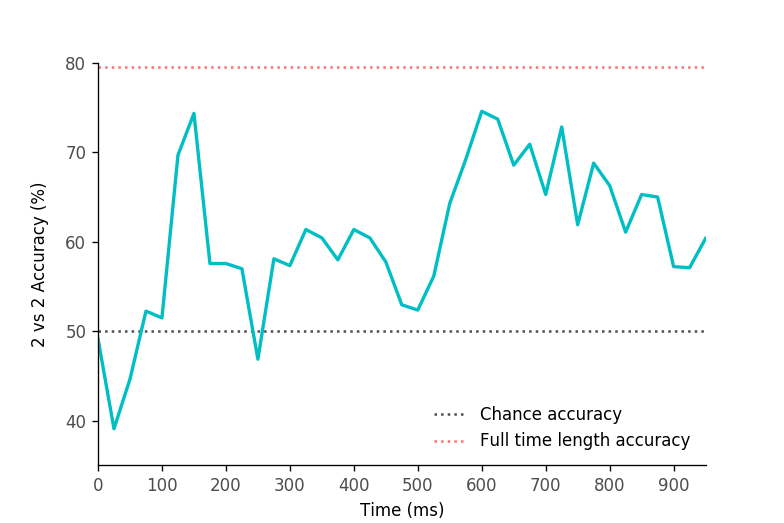
\includegraphics[width=0.75\linewidth]{figures/timewindow}
  \caption[\tvt Accuracy over Time]{
    A graph of 2 vs 2 accuracy over time. This graphic shows scores on the 2 vs 
    2 test evaluated with only the data present in 50ms incremental windows.  
    For example, the point at 25ms defines the \tvt accuracy over the 25ms-75ms 
    period. Statistically significant time windows are identified in red. The 
    highest performing period is 600-650ms with 74.57\% accuracy ($p < 0.001$, 
    FDR corrected). We also see an earlier spike which peaks at 150ms-200ms 
    with 74.3\% accuracy ($p < 0.001$, FDR corrected).
  }
  \label{fig:timewindow}
\end{figure}

The Time Windowing Experiment allows us to examine when the semantic 
representation in the brain is the strongest. The \tvt accuracy as a function 
of time \emph{within} an exposure is shown in Figure \ref{fig:timewindow}, 
allowing us to pinpoint the window where accuracy peaks. We find accuracy peaks 
in the 600ms-650ms window, at 74.57\% ($p < 0.001$, FDR corrected). We also see 
an earlier spike which peaks in the 150ms-200ms window, at 74.34\% ($p < 
0.001$, FDR corrected).

The later peak confirms our hypothesize, which was that we would see a delayed
peak due to the cognitive requirement of translating from the symbol to the 
English word before the semantics of the English word can be represented.  
However, we were surprised to see a strong early peak in the semantic 
representation. There is some evidence of an early semantic representation 
signal in other work, which is discussed in more detail in 
Section~\ref{sec:results:timewindowing}.
